\documentclass{beamer}
\usepackage[utf8]{inputenc}
\usepackage[autostyle]{csquotes}
\usepackage{fancybox}
\usepackage{graphicx}
\usepackage{hyperref}
%\usepackage{subcaption}
\usepackage{tabulary}
\usepackage{tabularx}
\usepackage[export]{adjustbox}
%\usepackage[style=numeric]{biblatex}
%\addbibresource{library.bib}
 
 
\title{Yubikey Wat is dat? Wat kann dat?}
\author{judge}
\date{}

\usetheme{metropolis}
\usecolortheme{default}

\begin{document}
 
\frame{\titlepage}

%\section{One Key to rule them all}
\begin{frame}
\frametitle{One Key to rule them all}
	\begin{figure}[h]
		\center
		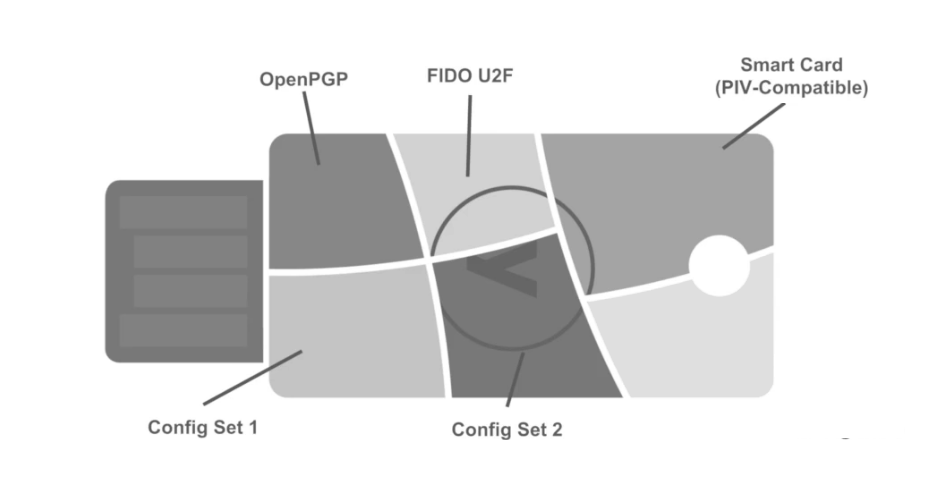
\includegraphics[width=0.7\textwidth]{images/functionality.png}
	\end{figure}
	\begin{columns}
		\column{0.33\textwidth}
			\pause
			\textbf{Config Slots}
			\begin{itemize}
				\item<3->{Synchrone Verschlüsselung}
				\item<3->{Yubico OTP}
				\item<3->{HOTP}
				\item<3->{Challenge Response}
			\end{itemize}
		\column{0.33\textwidth}
			\textbf{PGP Smartcard}
			\begin{itemize}
				\item<4->{Asynchrone Verschlüsselung}
				\item<4->{Encryption}
				\item<4->{Signing}
				\item<4->{Authentication}
			\end{itemize}
		\column{0.33\textwidth}
			\textbf{PIV Smartcard}
			\begin{itemize}
				\item<5->{Asynchrone Verschlüsselung}
				\item<5->{4 Slots usable for multiple purposes}
			\end{itemize}
	\end{columns}
\end{frame}

\begin{frame}
\frametitle{Second Factor}
	\begin{columns}
		\column{0.5\textwidth}
			\textbf{Website Login}
				\begin{itemize}
					\item{Yubico OTP}
					\item{generate OTP with yubikey, gets validated agains yubico cloud (they need to know the symmetric key)}
				\end{itemize}
		\pause
		\column{0.5\textwidth}
			\textbf{Password Manager}
				\begin{itemize}
					\item{Using Challenge Response}
					\item{KeepassXC (or KeepassX with Plugin)}
					\item{hash of database, as input to challenge, result gets appended to pasword}
				\end{itemize}
	\end{columns}
\end{frame}

\begin{frame}
\frametitle{Second Factor}
	\textbf{HOTP}
		\begin{itemize}
			\item{Google Authentication (TOTP)}
			\item{TOTP basiert HTOP}
			\item{Synchrone keys werden auf yubikey gelegt}
			\item{Generierung der keys mit app sowohl auf android als auch linux}
		\end{itemize}
\end{frame}

\begin{frame}
\frametitle{Rechner login}
	\begin{itemize}
		\item{Using PIV Smartcard}
		\item{Sign Challenge with Private Key}
		\item{OpenSC + PAM \url{https://github.com/OpenSC/pam_p11}}
	\end{itemize}
\end{frame}

\begin{frame}
\frametitle{SSH Authentication}
	\begin{itemize}
		\item{Export PGP Public key as SSH key}
		\item{Use gpg-agent als ssh-agent}
	\end{itemize}
\end{frame}

\end{document}

